\section{Supplementary Material}
\label{sec:supplementary_material}

\subsection{Derivation of the SOS constraints \cref{eq:sos_constraint_incompatible}} \label{sec:derive_sos_constr}

The objective of this section is to convert the empty-set condition \cref{eq:empty-set_conditions_clf} into the SOS constraint given in \cref{eq:sos_constraint_incompatible_clf}. The derivation of \cref{eq:sos_constraint_incompatible_cbf} and \cref{eq:sos_constraint_incompatible_cbf_un} is analogous.
Applying Putinar's P-satz to \cref{eq:empty-set_conditions_clf} yields the SOS constraint
\begin{align*}
   &-\nabla V^T f - d \in \textbf M(\nabla V^T G, -\nabla V^T G, V, -B_{\mathcal I_t}).
\end{align*}
By utilizing the definition of a quadratic module in \cref{eq:quadratic_module}, we can express this SOS constraint by the condition that there exist two SOS polynomials $p_{0,1}, p_{0,2} \in (\Sigma[x])^m$ such that
\begin{align*}
   &-\nabla V^T \left ( f + G (p_{0,1} - p_{0,2}) \right ) - d \in \textbf M(V, -B_{\mathcal I_t}).
\end{align*}
By exploiting the fact that the set of SOS polynomials, when combined with the set of negative SOS polynomials, spans the entire set of polynomials (i.e., $\Sigma[x] - \Sigma[x] = R[x]$), we can reformulate the SOS constraint as the condition that there exists a polynomial $p_0 \in (R[x])^m$ such that
\begin{align*}
   &-\nabla V^T \left ( f + G p_0 \right ) - d \in \textbf M(V, -B_{\mathcal I_t}).
\end{align*}
Finally, we introduce an additional SOS polynomial $s_0(x)$ (cf. \cref{eq:putinars_psatz_sos_condition}) and rewrite the SOS constraint as the condition that there exists $s_0 \in \Sigma[x], p_0 \in (R[x])^m$ such that
\begin{align*}
   &-\nabla V^T \left ( s_0 f + G p_0 \right ) - s_0 d \in \textbf M(V, -B_{\mathcal I_t}).
\end{align*}
The introduction of the polynomial $s_0(x)$ increases the set of feasible solutions when truncating the degrees of the involved polynomials, as described in \cref{sec:putinars_psatz}.



\subsection{Lower and upper bounds of $r_0(x)$}

   \begin{figure}[!t]
      \centering
      \resizebox{80mm}{!}{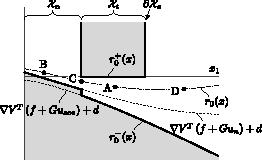
\includegraphics{images/10_upper_and_lower_bound.pdf}}
      \caption{(Upper and lower bounds on $r_0(x)$):
         Whereas the upper bound $r_0^+(x)$ is directly given by the CLF condition in \cref{eq:clf_condition}, only an estimate of the lower bound $r_0^-(x)$ can be obtained by the solution of the SOS constraints in \cref{eq:sos_opt_prob} involving $u_\text{sos} := p(x) / s(x)$ and the legacy controller $u_n(x)$.
      }
      \label{fig:bounds_on_ri}
   \end{figure}

   We illustrate a typical design choice for $r_0(x)$, as defined in \cref{eq:qcqp_based_controller}, in \cref{fig:bounds_on_ri}.

   For states inside the transitional region $x \in \mathcal X_t$ (see point \textbf{A} in \cref{fig:bounds_on_ri}), $r_0(x)$ is required to be smaller than the upper bound $r_0^+(x) = 0$ for \cref{eq:qcqp_based_controller_constraints} to satisfy the CLF condition in \cref{eq:clf_condition}.
   On the other hand, an estimate of the lower bound on $r_0(x)$ can be obtained from the solution $u_\text{sos}(x) = p(x)/s(x)$ of the SOS problem in \cref{eq:sos_opt_prob}.
   The corresponding lower bound is then given by $r_0^-(x) = \nabla V(x)^T \left ( f(x) + G(x) u_\text{sos}(x) \right ) + d(x)$, which is smaller than the upper bound $r_0^+(x) = 0$ within $\mathcal X_t$ due to \cref{eq:sos_constraint_inequality_clf}.
   We wish to emphasize that there may exist more optimal lower bounds on $r_0(x)$; however, the one chosen is certified by the SOS constraints developed in the previous chapter.

   For states inside the nominal region $x \in \mathcal X_n$ (see point \textbf{B} in \cref{fig:bounds_on_ri}), no upper bound is specified.
   Hence, by selecting a large $r_0(x)$, we can relax the corresponding constraint of the QCQP in \cref{eq:qcqp_based_controller_constraints}.
   Applying the same approach to other $r_i(x)$ allows us to enlarge the feasible set until $u := u_n(x)$ is a feasible solution for the QCQP, required to satisfy \cref{eq:sf_inactive_condition}.
   Therefore, we propose the following lower bound: $r_0^-(x) = \nabla V(x)^T \left ( f(x) + G(x) u_{n}(x) \right ) + d(x)$.
   By assigning $u := u_n(x)$, the corresponding constraint of the QCQP, expressed as $r_0^-(x) - r_0(x) \leq 0$, is clearly satisfied.

   For states on the boundary of the nominal region $x \in \partial \mathcal X_n$ (see point \textbf{C} in \cref{fig:bounds_on_ri}), we must ensure compatibility of the lower and upper bounds discussed in the previous paragraphs.
   More concretely, we need to ensure that $\nabla V(x)^T \left ( f(x) + G(x) u_{n}(x) \right ) + d(x) \leq 0$ for all $x \in \partial \mathcal X_n$.
   However, this inequality follows directly from inequality \cref{eq:sos_constraint_inequality_nom}.

   Finally, for states outside the safe set $x \notin \mathcal X_s$ (see point \textbf{D} in \cref{fig:bounds_on_ri}), an upper bound on $r(x)$ is not specified.
   The lower bound can be chosen as in \textbf{A}.
   It is however important to note that the region can be made attracting with respect to the safe set by the additional requirement of selecting a negative $r(x)$.
   This can restore the system state to the safe set in scenarios where unexpected system noise or model mismatch cause the system to deviate from the safe set.



\subsection{Alternating Algorithm} \label{sec:algorithm}

The solution of the SOS problem \cref{eq:sos_opt_prob} presents a particular challenge due to its bilinearity, i.e., the simultaneous search for CBF $B(x)$, CLF $V(x)$, a rational controller $u_\text{SOS}(x)$, and other SOS polynomials introduced by the Positivstellensatz.
This bilinearity prevents us from converting the SOS problem directly into a Semi-Definite Program (SDP).
Similar to \cite{TanPackard:04,schneeberger2023sos}, however, we can iteratively alternate between searching over one set of decision variables while keeping the others fixed.
Such an alternating algorithm requires a feasible initialization of the decision variables that are kept fixed in the SDP of the first iteration.
Therefore, we propose an initialization procedure to find such an initial set of feasible parameters following the presentation of the main algorithm.



\subsection{Main algorithm} \label{sec:main_algorithm}

To make the main algorithm compatible with the initialization procedure, we introduce an \emph{operating region} that contains the allowable set $\mathcal X_a$:
\begin{align} \label{eq:radius_of_interest}
   \mathcal X_\text{op} := \{ x \mid f_\text{op}(x) \leq 0 \} \supseteq \mathcal X_a,
\end{align}
with scalar polynomial $f_\text{op} \in R[x]$.
We assume that there exists a constant $\rho_\Sigma \in \R$ such that 
\begin{align} \label{eq:rho_sigma}
   f_\text{op}(x) + \rho_\Sigma \in \Sigma[x]
\end{align}
is an SOS polynomial.
This assumption, while not overly restrictive, is important for establishing the feasibility of the SDP in \textit{Part 1} of the initialization procedure, as elaborated in the subsequent subsection.

\begin{remark}
   \textit{
      The operating region $\mathcal X_\text{op}$ can be determined by solving another SOS problem, as condition \cref{eq:rho_sigma} directly translates to an SOS constraint.
      By making minor adjustments, it is possible to define the operating region $\mathcal X_\text{op}$ using multiple polynomials, and it could even coincide with the allowable set $\mathcal X_a$.
      However, in order to reduce computational complexity, we restrict the number of polynomials to one.
      In cases, where the operating region $\mathcal X_\text{op}$ closely approximates the safe set $\mathcal X_s$, the polynomials $B_i(x)$ in the quadratic modules of the SOS problem in \cref{eq:sos_opt_prob} can be omitted, thereby reducing the total number of decision variables.
      This will reduce computational complexity by introducing slightly more conservative SOS constraints.
   }
\end{remark}

The constraint $f_\text{op}(x) \leq 0$ defining the operating region $\mathcal X_\text{op}$ is added to the empty set conditions \cref{eq:empty-set_conditions} developed in \cref{sec:sos_optimization}.
From a set-theoretic point of view, adding the constraint $f_\text{op}(x) \leq 0$ does not alter the empty set conditions, given that $\mathcal X_s \subseteq \mathcal X_\text{op}$.
However, by applying Putinar's P-satz on the empty set conditions \cref{eq:empty-set_conditions} including $f_\text{op}(x) \leq 0$, we obtain slightly different SOS constraints for all $i \in \mathcal I_t$:
\begin{subequations} \label{eq:sos_constraint_roi}
   \begin{align}
      \begin{split}
         &-\nabla V^T \left ( s f + G p \right ) - s d \in \textbf M(V, -B_{\mathcal I_t}, -f_\text{op})
      \end{split} \\
      \begin{split}
         &-\nabla B_i^T \left ( s f + G p \right ) \in \textbf M(B_i, -B_{\mathcal I_t}, -f_\text{op})  
      \end{split} \\
      \begin{split}
         &-\nabla V^T \left ( f + G u_n \right ) - d \in \textbf M(V, -V, -f_\text{op}).
      \end{split}
   \end{align}
\end{subequations}
These SOS constraints are used to define the main algorithm.

The main algorithm involves alternating between two SDPs, as described by \textit{Part 1} and \textit{Part 2} below.
Given an initial set of feasible parameters, the SDP in \textit{Part 1} is guaranteed to be feasible for each iteration when utilizing the solution from \textit{Part 2}.
Likewise, the SDP in \textit{Part 2} is guaranteed to be feasible for each iteration when utilizing the solution from \textit{Part 1}.
Furthermore, as shown in \cite{schneeberger2023sos}, the cost of the SDP in \textit{Part 1} encoding the volume of the safe set is non-decreasing over the iterations.



\subsubsection*{Part 1 - Searching for CBF and CLF}

In the first part, we search over CBFs $B_i(x)$ and a CLF $V(x)$ that maximize the volume of the safe set.
To make the SDP computationally tractable, we approximate the volume of the safe set by the summation of traces of $Q_{B_i}$, similar to \cite{WangHan:18,KunduGeng:19}:
\begin{align*} 
   \hspace{-\leftmargin}
   \begin{array}{lll}
      \mbox{find} & V, B_i \in R[x] \\
      \mbox{hold fixed} & p, s \\
      \mbox{maximize} & \sum_{i \in \mathcal I_t} tr(Q_{B_i}) \\
      \mbox{subject to} & \text{\cref{eq:sos_constraint_xs_subsetneq_xa,eq:sos_constraint_xn_subsetneq_xs,eq:sos_constraint_roi}}, \\
   \end{array}
\end{align*}
where the $Q_{B_i}$ are derived from the decomposition of the CBF $B_i(x)$ into $B_i(x) = Z_{B,i}(x)^T Q_{B,i} Z_{B,i}(x)$ (cf. \cref{eq:quadratic_matrix_form}).



\subsubsection*{Part 2 - Searching for a controller}

For the second part of the main algorithm, we search over a rational controller $u_\text{SOS}(x) = p(x)/s(x)$ that maximizes the SOS constraint margins, denoted by $\Delta_i \in \R$, $i \in \{ 0 \} \cup \mathcal I_t$.
Only the first two SOS constraints from \cref{eq:sos_constraint_roi} depend on the rational controller.
They are specified with the inclusion of these margins $\Delta_i$ as:
\begin{subequations} \label{eq:sos_constraint_margin}
   \begin{align}
      \begin{split}
         &-\nabla V^T \bigl ( s f + G p \bigr ) - s d + \Delta_0 \in \textbf M(B_i, -B_{\mathcal I_t}, -f_\text{op}) \\
      \end{split} \\
      \begin{split}
         &-\nabla B_i^T \bigl ( s f + G p \bigr ) + \Delta_i \in \textbf M(B_i, -B_{\mathcal I_t}, -f_\text{op})
      \end{split}
   \end{align}
\end{subequations}
for all $i \in \mathcal I_t$.
Large values of $\Delta_i$, $i \in \{ 0 \} \cup \mathcal I_t$, will increase the set of feasible solution in \textit{Part 1} in the subsequent iterations.
The SDP involved in \textit{Part 2} is given by:
\begin{align} \label{eq:sos_opt_prob_part2}
   \hspace{-\leftmargin}
   \begin{array}{lll}
      \mbox{find} & p \in (\R[x])^m, s \in \Sigma[x], \Delta_i \in \R \\
      \mbox{hold fixed} & V, B_i \\
      \mbox{maximize} & \sum_{i \in \{0\} \cup \mathcal I_t} \Delta_i \\
      \mbox{subject to} & \text{\cref{eq:linear_input_sos_constraints,eq:quadratic_input_constraints,eq:sos_constraint_margin}} \\
      & s - \epsilon \in \Sigma[x], \Delta_\text{min} \leq \Delta_i.
   \end{array}
\end{align}
A constant $\epsilon > 0$ assures that $s(x) > 0$.
The minimum margin $\Delta_\text{min} < 0$ is selected to maintain numerical stability of the algorithm.
The main algorithm concludes when the increment in $\sum_{i \in \mathcal I_t} tr(Q_{B_i})$ in \textit{Part 1} does not exceed a predefined minimal threshold.



\subsection{Initialization procedure} \label{sec:init_procedure}

\begin{figure}[!t]
   \centering
   \resizebox{85mm}{!}{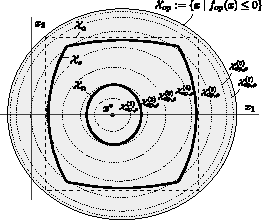
\includegraphics{images/11_growing_region_of_interest}}
   \caption{(Operating region):
      The initialization procedure produces an initial set of feasible parameters for the main algorithm by iteratively expanding the operating region $\mathcal X_{\text{op},\rho}$.
      The initialization procedure finishes 
      if $\mathcal X_\text{op} = \mathcal X_{\text{op},\rho}^{(k)}$.
   }
   \label{fig:growing_region_of_interest}
\end{figure}

The main algorithm, presented in previous subsection, requires an initial set of feasible parameters.
Therefore, we present an initialization procedure to find such an initial set.

Similar to the main algorithm, the initialization procedure involves an alternating between two SDPs, as described by \textit{Part 1} and \textit{Part 2} below.
The feasibility of each part is guaranteed by employing the solution of the SDP from the previous iteration.
To make sure that the SDP in \textit{Part 1} is feasible in the first iteration, we use a modified operating region (cf. \cref{eq:radius_of_interest})
\begin{align} \label{eq:small_radius_of_interest}
   \mathcal X_{\text{op}, \rho} := \{ x \mid f_\text{op}(x) + \rho \leq 0 \},
\end{align}
with $\rho \geq 0$.
By choosing the $\mathcal X_{\text{op}, \rho}$ initially sufficiently small in volume, i.e., a large $\rho > 0$, we guarantee feasibility of the SDP in \textit{Part 1} for any initial set of parameters, as shown in \cref{lem:feasible_solution}.

By applying Putinar's P-satz on the modified empty set condition \cref{eq:empty-set_conditions} including $f_\text{op} + \rho \leq 0$ instead, we derive the following SOS constraints for all $i \in \mathcal I_t$:
\begin{subequations} \label{eq:sos_constraint_init_roi}
   \begin{align}
      \begin{split}
         &-\nabla V^T \left ( s f + G p \right ) - s d \in \textbf M(V, -B_{\mathcal I_t}, f_\text{op} + \rho)
      \end{split} \\
      \begin{split}
         &-\nabla B_i^T \left ( s f + G p \right ) \in \textbf M(B_i, -B_{\mathcal I_t}, f_\text{op} + \rho)  
      \end{split} \\
      \begin{split}
         &-\nabla V^T \left ( f + G u_n \right ) - d \in \textbf M(V, -V, f_\text{op} + \rho).
      \end{split}
   \end{align}
\end{subequations}



\subsubsection*{Part 1 - Searching for CBF and CLF}

The first part of the initialization procedure searches over CBF and a CLF that maximize $\rho$, thereby increasing the volume of $\mathcal X_{\text{op}, \rho}$ for every iteration (cf. \cref{fig:growing_region_of_interest}).
To make sure that $\mathcal X_{\text{op}, \rho}$ is contained in the operating region, i.e., $\mathcal X_\rho^{(k)} \subseteq \mathcal X_\text{op}$, we impose the constraint that $0 \leq \rho$.
The resulting SDP is expressed as:
\begin{align} \label{eq:sos_opt_prob_part1}
   \hspace{-\leftmargin}
   \begin{array}{lll}
      \mbox{find} & V, B_i \in R[x], \rho \in \R \\
      \mbox{hold fixed} & p, s \\
      \mbox{maximize} & \rho \geq 0 \\
      \mbox{subject to} & \text{\cref{eq:sos_constraint_xs_subsetneq_xa,eq:sos_constraint_xn_subsetneq_xs,eq:sos_constraint_init_roi}}. \\
   \end{array}
\end{align}

The next lemma establishes feasibility of the SDP \cref{eq:sos_opt_prob_part1} in the first iteration.
Its proof can be found in the appendix.
\begin{lemma} \label{lem:feasible_solution}
   Assuming that there exist candidates $V(x)$ and $B_i(x)$ that satisfy conditions \cref{eq:sos_constraint_xs_subsetneq_xa,eq:sos_constraint_xn_subsetneq_xs}, then the SDP in \cref{eq:sos_opt_prob_part1} is feasible using random initial coefficient values for polynomials $p(x) \in (R[x])^m$ and $s(x) \in \Sigma[x]$.
\end{lemma}
\begin{IEEEproof}
   By utilizing the definition of a quadratic module in \cref{eq:quadratic_module}, the conditions in \cref{eq:sos_constraint_init_roi} can be formulated as the existence of $\gamma_{0,i}, \gamma_n \in R[x]$, $\gamma_{0,0}, \gamma_{\text{op}, 0}, \gamma_{\text{op},i}, \gamma_{\text{op},n} \in \Sigma[x]$, and $\gamma_{1,i}, \gamma_{1,0} \in (\Sigma[x])^t$ such that
   \begin{subequations} \label{eq:sos_constraint_lemma_4}
      \begin{align}
         \begin{split}
            & q_i + \gamma_{\text{op}, i} (f_\text{op} + \rho) \in \Sigma[x]   
         \end{split} \\
         \begin{split}
            & q_0 + \gamma_{\text{op}, 0} (f_\text{op} + \rho) \in \Sigma[x]
         \end{split} \\
         \begin{split}
            & q_n + \gamma_{\text{op}, n} (f_\text{op} + \rho) \in \Sigma[x],
         \end{split}
      \end{align}
   \end{subequations}
   with polynomials \begin{itemize}
      \item $q_i := -\nabla B_i^T \left ( s f + G p \right ) - \gamma_{0,i} B_i + \gamma_{1,i}^T B_{\mathcal I_t}$
      \item $q_0 := -\nabla V^T \left ( s f + G p \right ) - s d - \gamma_{0,0} V + \gamma_{1,0}^T B_{\mathcal I_t}$
      \item $q_n := -\nabla V^T \left ( f + G u_n \right ) - d + \gamma_n V$.
   \end{itemize}
   
   First, we show that for any polynomial $q \in R[x]$, we can find $\gamma_{\text{op}} \in \Sigma[x]$ and $\rho \in \R$ such that
   \begin{align} \label{eq:abstract_q_sos}
      q(x) + \gamma_{\text{op}}(x) (f_\text{op}(x) + \rho ) \in \Sigma[x].
   \end{align}
   To show this, we select an SOS polynomial $\gamma_{\text{op}} \in \Sigma[x]$ sufficiently large such that $q(x) + \gamma_{\text{op}}(x) \in \Sigma[x]$.
   This is always possible since starting from the decomposition $q(x) = Z(x)^T Q_f Z(x)$ (cf. \cref{eq:quadratic_matrix_form}), we can select $\gamma_{\text{op}}(x) = \nu Z(x)^T Z(x)$, with arbitrary large $\nu > 0$, such that $Q_f + \nu I \succcurlyeq 0$.
   Second, by utilizing the assumption on $\rho_\Sigma$ (cf. \cref{eq:rho_sigma}), choose $\rho := \rho_\Sigma + 1$ such that
   $q(x) + \gamma_{\text{op}}(x) + \gamma_{\text{op}}(x) (\rho(x) + \rho_\Sigma ) \in \Sigma[x]$.
   Hence, any $\rho \geq \rho_\Sigma + 1$ renders \cref{eq:abstract_q_sos} an SOS polynomial.
   
   In this way, we can find $\rho$ for each SOS constraint in \cref{eq:sos_constraint_lemma_4}, and denote them by $\rho_0, \rho_i, \rho_n \in \R$.
   By selecting $\rho := max(\rho_0, \rho_i, \rho_n)$, all SOS constraints in \cref{eq:sos_constraint_lemma_4} hold simultaneously.
   Hence, the SOS problem \cref{eq:sos_opt_prob_part1} is feasible for any initialization of $q_0(x)$, $q_i(x)$, $i \in \mathcal I_t$, and $q_n(x)$.
\end{IEEEproof}



\subsubsection*{Part 2 - Searching for a controller}

Similar to the main algorithm, we search over a rational controller $u_\text{SOS}(x) = p(x)/s(x)$ that maximizes the SOS constraint margins, denoted by $\Delta_i \in \R$, $i \in \{ 0 \} \cup \mathcal I_t$.
The corresponding SOS constraints including these margins $\Delta_i$ are specified as:
\begin{subequations} \label{eq:sos_constraint_init_margin}
   \begin{align}
      \begin{split}
         &-\nabla V^T \left ( s f + G p \right ) - d + \Delta_0 \in \textbf M(V, -B_{\mathcal I_t}, f_\text{op} + \rho)
      \end{split} \\
      \begin{split}
         &-\nabla B_i^T \left ( s f + G p \right ) + \Delta_i \in \textbf M(B_i, -B_{\mathcal I_t}, f_\text{op} + \rho),
      \end{split}
   \end{align}
\end{subequations}
for all $i \in \mathcal I_t$.
The resulting SDP is given by:
\begin{align*}
   \hspace{-\leftmargin}
   \begin{array}{lll}
      \mbox{find} & p \in (\R[x])^m, s \in \Sigma[x], \Delta_i \in \R \\
      \mbox{hold fixed} & V, B_i, \rho \\
      \mbox{maximize} & \sum_{i \in \{0\} \cup \mathcal I_t} \Delta_i \\
      \mbox{subject to} & \text{\cref{eq:linear_input_sos_constraints,eq:quadratic_input_constraints,eq:sos_constraint_init_margin}}, \\
      & s - \epsilon \in \Sigma[x], \Delta_\text{min} \leq \Delta_i.
   \end{array}
\end{align*}
A constant $\epsilon > 0$ assures that $s(x) > 0$.
Similar to the SDP \cref{eq:sos_opt_prob_part2}, the minimum margin $\Delta_\text{min} < 0$ is selected to maintain numerical stability of the algorithm.
The initialization procedure is considered complete when $\rho = 0$, i.e., $\mathcal X_\rho^{(k)} = \mathcal X_\text{op}$.
At this point, we found an initial set of feasible parameters for the SDP in \textit{Part 1} of the main algorithm.
\begin{remark}
   \textit{
      The initialization procedure can be extended with additional steps where the margins $\Delta_i$ are introduced when searching over the controller, or the operational region is expanded -- by decreasing $\rho$ -- when searching for CBF and CLF. 
      Furthermore, we can introduce additional steps where we optimize only over a subset of the $\Delta_i$'s.
   }
\end{remark}